\section{具体运输问题}
\label{sec:ot-concrete}

前两节回答了最优耦合何时存在、怎样证实。真正把它求出来，要靠问题本身的结构。本节看三类结构：实数轴上的顺序使最优方案“不交叉”，可以由分位数直接写出；有限支持使问题成为线性规划；高斯分布与平方成本的二次结构使最优方案是一个仿射映射。每个问题都要回答两件事：最优成本是多少，以及最优方案是一般耦合还是由映射产生。

\subsection{一维分布}
\label{sec:ot-one-dimensional}

在实数轴上，交叉的搬运总是浪费。设$x_1<x_2$两处各有一份质量，要送到$y_1<y_2$。交叉配对把$x_1$送到$y_2$、$x_2$送到$y_1$，顺序配对则$x_1\to y_1$、$x_2\to y_2$，见图~\ref{fig:ot-uncross}。对凸的成本$h(x-y)$，顺序配对不会更贵：交叉配对的两个位移$x_1-y_2$与$x_2-y_1$一个最小、一个最大，顺序配对的两个位移夹在中间且总和相同，凸函数在两端的和不小于在中间的和。这启发我们：最优方案应当按顺序配对，把源分布的第$u$分位数送到目标分布的第$u$分位数。

\begin{BookInlineFigure}
 \centering
 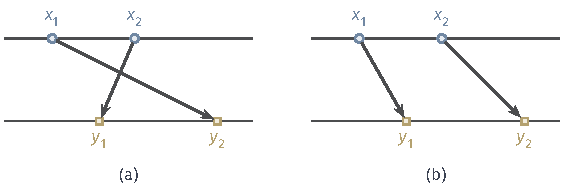
\includegraphics[width=96mm]{figures/07-probability/07-distribution-optimization/tikz/ot-uncross/figure.pdf}
 \caption{实数轴上的交换论证。上方是源点$x_1<x_2$（蓝），下方是目标点$y_1<y_2$（黄）。(a)交叉配对。(b)顺序配对。对凸成本$h(x-y)$，(b)的成本不超过(a)。}
 \label{fig:ot-uncross}
\end{BookInlineFigure}

\paragraph{分位数耦合}
设$\mu,\nu$是实数轴上的分布，分布函数为$F,G$。沿用第~\ref{chap:random-variables}章的广义分位数$F^{-1}(u)=\inf\{x:F(x)\geq u\}$，$0<u<1$，它满足
\[
 F^{-1}(u)\leq x\quad\Longleftrightarrow\quad u\leq F(x).
\]
取$U\sim\operatorname{Unif}(0,1)$，令$X=F^{-1}(U)$，$Y=G^{-1}(U)$。由上面的等价关系，$\mathbb{P}(X\leq x)=\mathbb{P}(U\leq F(x))=F(x)$，所以$X\sim\mu$；同理$Y\sim\nu$。$(X,Y)$的联合分布因此是$\mu$与$\nu$的一个耦合，称为\term{分位数耦合}（quantile coupling）。它的联合分布函数是
\begin{equation}
 \mathbb{P}(X\leq s,\ Y\leq t)=\mathbb{P}\bigl(U\leq F(s),\ U\leq G(t)\bigr)=\min\bigl(F(s),G(t)\bigr).
 \label{eq:ot-comonotone-cdf}
\end{equation}
两个分量由同一个$U$单调地决定，$U$越大两者都越大，所以这个耦合“不交叉”。

\begin{theorem}[一维最优运输]
\label{thm:ot-one-dimensional}
设$\mu,\nu$是实数轴上具有有限$p$阶矩的分布，$p\geq1$，分布函数为$F,G$，成本$c(x,y)=\lvert x-y\rvert^{p}$。则分位数耦合是最优耦合，
\begin{equation}
 W_p^{p}(\mu,\nu)=\int_0^{1}\bigl\lvert F^{-1}(u)-G^{-1}(u)\bigr\rvert^{p}\,\mathrm{d}u .
 \label{eq:ot-quantile-formula}
\end{equation}
$p=1$时还有
\begin{equation}
 W_1(\mu,\nu)=\int_{-\infty}^{\infty}\bigl\lvert F(x)-G(x)\bigr\rvert\,\mathrm{d}x .
 \label{eq:ot-cdf-formula}
\end{equation}
$p>1$时最优耦合唯一。
\end{theorem}

$p=1$与$p>1$的证明思路不同。$p=1$时成本对距离是线性的，可以把$\lvert x-y\rvert$拆成对阈值的积分，直接得到下界；$p>1$时先由第~\ref{sec:ot-existence}节取得一个最优耦合，再证明它必定不交叉，不交叉的耦合只有分位数耦合一个。

\begin{proof}[$p=1$的证明]
对实数$x,y$，示性函数$\mathbf{1}_{\{x\leq t\}}$与$\mathbf{1}_{\{y\leq t\}}$只在$t$介于$x,y$之间时不同，所以
\[
 \lvert x-y\rvert=\int_{-\infty}^{\infty}\bigl\lvert\mathbf{1}_{\{x\leq t\}}-\mathbf{1}_{\{y\leq t\}}\bigr\rvert\,\mathrm{d}t .
\]
任取耦合$(X,Y)$，两边取期望，被积函数非负，由Tonelli定理交换期望与积分，再对每个$t$用“绝对值的期望不小于期望的绝对值”，
\[
 \mathbb{E}\lvert X-Y\rvert=\int_{-\infty}^{\infty}\mathbb{E}\bigl\lvert\mathbf{1}_{\{X\leq t\}}-\mathbf{1}_{\{Y\leq t\}}\bigr\rvert\,\mathrm{d}t\geq\int_{-\infty}^{\infty}\lvert F(t)-G(t)\rvert\,\mathrm{d}t .
\]
所以式~\eqref{eq:ot-cdf-formula}右边是一切耦合成本的下界。

对分位数耦合，$\{X\leq t\}=\{U\leq F(t)\}$，$\{Y\leq t\}=\{U\leq G(t)\}$，两个事件一个包含另一个，所以
\[
 \mathbb{E}\bigl\lvert\mathbf{1}_{\{X\leq t\}}-\mathbf{1}_{\{Y\leq t\}}\bigr\rvert=\bigl\lvert F(t)-G(t)\bigr\rvert ,
\]
上面的不等式取等。分位数耦合达到下界，是最优耦合，并且$W_1$同时等于式~\eqref{eq:ot-quantile-formula}与式~\eqref{eq:ot-cdf-formula}的右边。
\end{proof}

式~\eqref{eq:ot-cdf-formula}说的是：$W_1$等于两条分布函数曲线之间的面积。式~\eqref{eq:ot-quantile-formula}说的是同一块面积换一个方向切片：按纵坐标$u$切成水平条，每条的长度是$\lvert F^{-1}(u)-G^{-1}(u)\rvert$。图~\ref{fig:ot-quantile-coupling}对全章例子画出两种看法。

$p>1$的证明需要一个关于最优耦合支撑的引理。$\mathbb{R}^{2}$上分布$\pi$的支撑是这样的点$z$的全体：以$z$为中心的每个开球都有正的$\pi$质量。支撑之外的点各有一个零质量邻域，这些邻域可以由可数个有理中心、有理半径的零质量球覆盖，所以支撑之外的总质量为零；换句话说，正质量的集合一定与支撑相交。

\begin{lemma}[最优耦合不能局部改进]
\label{lem:ot-two-point}
设$c:\mathbb{R}\times\mathbb{R}\to[0,\infty)$连续，$\pi$是$\mu,\nu$的成本有限的最优耦合。则对$\pi$支撑中的任意两点$(x_1,y_1),(x_2,y_2)$，
\begin{equation}
 c(x_1,y_1)+c(x_2,y_2)\leq c(x_1,y_2)+c(x_2,y_1).
 \label{eq:ot-two-point}
\end{equation}
\end{lemma}

\begin{proof}
设两点不同而不等式反向，差为$3\eta>0$。由连续性，可取$\delta>0$，使两个开方块
\[
 Q_k=(x_k-\delta,x_k+\delta)\times(y_k-\delta,y_k+\delta),\qquad k=1,2
\]
互不相交，并且只要$(x,y)\in Q_1$，$(x',y')\in Q_2$，就有
\[
 c(x,y)+c(x',y')\geq c(x,y')+c(x',y)+\eta .
\]
两点在支撑中，$m_k=\pi(Q_k)>0$。记$\pi_k=\pi|_{Q_k}/m_k$，它的两个边缘为$\alpha_k,\beta_k$。取$\lambda=\min(m_1,m_2)$，构造
\[
 \pi'=\pi-\lambda(\pi_1+\pi_2)+\lambda\bigl(\alpha_1\otimes\beta_2+\alpha_2\otimes\beta_1\bigr).
\]
在$Q_k$上$\pi\geq m_k\pi_k\geq\lambda\pi_k$，所以$\pi'$非负。第一边缘先减去$\lambda(\alpha_1+\alpha_2)$、再加回$\lambda(\alpha_1+\alpha_2)$，没有改变，第二边缘同理，于是$\pi'\in\Pi(\mu,\nu)$。这一步把两块中的质量“交换目的地”：$Q_1$里的源送往$Q_2$里的目标，反之亦然。成本的改变量是
\[
 \begin{aligned}
 &\lambda\iint\bigl(c(x,y')+c(x',y)-c(x,y)-c(x',y')\bigr)\,\pi_1(\mathrm{d}x,\mathrm{d}y)\,\pi_2(\mathrm{d}x',\mathrm{d}y')\\
 &\qquad\leq-\lambda\eta<0 ,
 \end{aligned}
\]
其中各项积分有限，因为$c$在有界集上有界。这与$\pi$最优矛盾。
\end{proof}

\begin{proof}[$p>1$的证明]
有限$p$阶矩保证独立耦合的成本有限，成本连续，由定理~\ref{thm:ot-existence}，最优耦合存在。任取一个最优耦合$\pi$，我们证明它就是分位数耦合，于是分位数耦合最优，而且最优耦合唯一。

\emph{第一步：支撑不交叉。}设支撑中有$(x_1,y_1),(x_2,y_2)$满足$x_1<x_2$而$y_1>y_2$。记
\[
 r=x_1-y_1,\qquad v=x_1-y_2,\qquad w=x_2-y_1,\qquad z=x_2-y_2 .
\]
则$v,w$都严格介于$r$与$z$之间，并且
\[
 v+w=r+z .
\]
令$\lambda=(z-v)/(z-r)\in(0,1)$，则
\[
 v=\lambda r+(1-\lambda)z,\qquad w=(1-\lambda)r+\lambda z .
\]
$h(s)=\lvert s\rvert^{p}$在$p>1$时严格凸，所以
\[
 h(v)+h(w)<\lambda h(r)+(1-\lambda)h(z)+(1-\lambda)h(r)+\lambda h(z)=h(r)+h(z),
\]
即$c(x_1,y_2)+c(x_2,y_1)<c(x_1,y_1)+c(x_2,y_2)$，与引理~\ref{lem:ot-two-point}矛盾。所以支撑中$x_1<x_2$蕴含$y_1\leq y_2$。

\emph{第二步：不交叉决定联合分布。}任取$s,t$。若事件$\{x\leq s,\,y>t\}$与$\{x>s,\,y\leq t\}$的$\pi$质量都为正，两者都与支撑相交，得到支撑中的点$(x_1,y_1)$、$(x_2,y_2)$，满足$x_1\leq s<x_2$且$y_2\leq t<y_1$，与第一步矛盾。所以两者至少有一个质量为零。若前者为零，
\[
 \pi(x\leq s,\,y\leq t)=\pi(x\leq s)=F(s),
\]
又因为它不超过$\pi(y\leq t)=G(t)$，它等于$\min(F(s),G(t))$。后者为零时同理。于是$\pi$的联合分布函数就是式~\eqref{eq:ot-comonotone-cdf}，二维分布由联合分布函数唯一确定，$\pi$等于分位数耦合。
\end{proof}

$p=1$时最优耦合一般不唯一。第~\ref{chap:distribution-comparison}章已经看到，例表上逐格搬运与跳格搬运的一阶成本相同；这正是$h(s)=\lvert s\rvert$不严格凸的结果，交换论证中的不等式可以取等。

\paragraph{例子的计算}
全章例子的两个分布函数与分位数函数分别是阶梯函数。$F$在$0,1,2$处跳到$0.5,0.8,1$，$G$跳到$0.2,0.5,1$。把$(0,1)$按两组跳跃高度切开，得到四个区间：
\[
 (0,0.2],\qquad(0.2,0.5],\qquad(0.5,0.8],\qquad(0.8,1).
\]
在这四段上$(F^{-1}(u),G^{-1}(u))$依次取$(0,0)$、$(0,1)$、$(1,2)$、$(2,2)$，各段长度$0.2,0.3,0.3,0.2$就是分位数耦合放在这些点对上的质量，它正是图~\ref{fig:ot-plan-tables}(c)的逐格搬运。由定理~\ref{thm:ot-one-dimensional}，逐格搬运是平方成本下唯一的最优方案，这印证了上一节用对偶势得到的结论。由式~\eqref{eq:ot-cdf-formula}，
\[
 W_1=\int_0^{1}(0.5-0.2)\,\mathrm{d}x+\int_1^{2}(0.8-0.5)\,\mathrm{d}x=0.6 ,
\]
这证明了第~\ref{chap:distribution-comparison}章提到的关系：$W_1$等于两条分布函数之间的面积。由式~\eqref{eq:ot-quantile-formula}，
\[
 W_2^{2}=0.3\times1^{2}+0.3\times1^{2}=0.6 .
\]

\begin{BookInlineFigure}
 \centering
 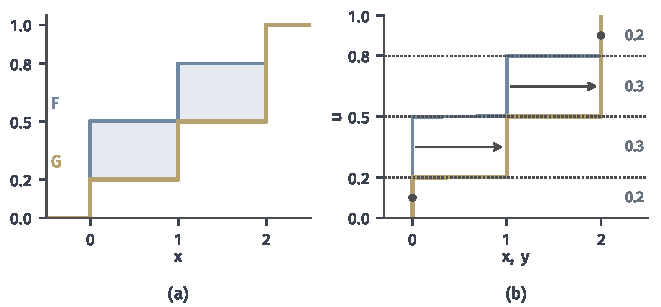
\includegraphics[width=112mm]{figures/07-probability/07-distribution-optimization/matplotlib/ot-quantile-coupling/figure.pdf}
 \caption{全章例子的一维运输。(a)$F$（蓝）与$G$（黄），两者之间浅蓝区域的面积是$W_1=0.6$。(b)分位数函数，横轴为取值，纵轴为$u$；虚线把$(0,1)$分成四段，每段内箭头从$F^{-1}(u)$指向$G^{-1}(u)$，右侧数字是该段长度，即搬运的质量；黑点表示质量留在原地。}
 \label{fig:ot-quantile-coupling}
\end{BookInlineFigure}

\paragraph{何时由映射实现}
分位数耦合是$U$的函数对，但不一定是$X$的函数。若$F$连续，它是。先说明$F(X)\sim\operatorname{Unif}(0,1)$：由分位数的等价关系，$F(x)\geq u$当且仅当$x\geq F^{-1}(u)$，而$F$连续时$\mathbb{P}(X=F^{-1}(u))=0$且$F(F^{-1}(u))=u$，所以
\[
 \mathbb{P}\bigl(F(X)\geq u\bigr)=\mathbb{P}\bigl(X\geq F^{-1}(u)\bigr)=1-u .
\]
再说明$F^{-1}(F(X))=X$几乎必然成立：总有$F^{-1}(F(x))\leq x$，严格小于只发生在$F$的平台上，平台的质量为零。于是取$U=F(X)$，分位数耦合就是$(X,\,G^{-1}(F(X)))$，
\begin{equation}
 T=G^{-1}\circ F
 \label{eq:ot-monotone-map}
\end{equation}
是一个单调不减的最优运输映射。

源分布有原子时，分位数耦合必须把原子拆开。取
\[
 \mu=\tfrac12\delta_0+\tfrac12\operatorname{Unif}(1,2),\qquad \nu=\operatorname{Unif}(0,2),
\]
则
\[
 F^{-1}(u)=\begin{cases}0, & u\leq\tfrac12,\\ 2u, & u>\tfrac12,\end{cases}\qquad G^{-1}(u)=2u .
\]
$u\leq\tfrac12$时，$0$处的原子被均匀地铺到$[0,1]$上；$u>\tfrac12$时质量不动。由式~\eqref{eq:ot-quantile-formula}，
\[
 W_1=\int_0^{1/2}2u\,\mathrm{d}u=\frac14,\qquad W_2^{2}=\int_0^{1/2}4u^{2}\,\mathrm{d}u=\frac16 .
\]
$W_1$也等于图~\ref{fig:ot-atom-quantile}(a)中$F$与$G$之间三角形的面积$\tfrac12\times1\times\tfrac12$。这里不存在任何运输映射：映射把$0$处质量为$\tfrac12$的原子整体送到一个点，像分布就有质量至少$\tfrac12$的原子，而$\nu$没有原子。分位数配对总能定义耦合，却未必给出源点的单值映射。

\begin{BookInlineFigure}
 \centering
 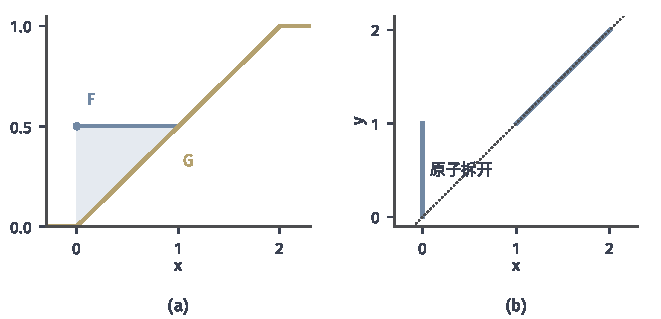
\includegraphics[width=112mm]{figures/07-probability/07-distribution-optimization/matplotlib/ot-atom-quantile/figure.pdf}
 \caption{带原子的源分布$\mu=\tfrac12\delta_0+\tfrac12\operatorname{Unif}(1,2)$与$\nu=\operatorname{Unif}(0,2)$。(a)$F$（蓝）与$G$（黄），在$[1,2]$上两者重合；浅蓝三角形面积$W_1=1/4$。(b)分位数耦合的支撑：$x=0$处的竖线表示原子被铺到$[0,1]$上，$[1,2]$上的斜线表示质量不动。}
 \label{fig:ot-atom-quantile}
\end{BookInlineFigure}

\subsection{离散运输}
\label{sec:ot-discrete}

高维的有限问题没有顺序可用，只能直接解线性规划。把$\bm{\pi}$排成长为$mn$的向量，问题是$m+n$个等式约束、$mn$个非负变量的线性规划。行约束之和与列约束之和都等于总质量$1$，所以等式约束中有一个是多余的，独立的约束是$m+n-1$个。

\paragraph{顶点的结构}
由前面提到的线性规划理论，线性规划若有最优解，就有一个最优解是可行集合的顶点。运输多面体的顶点有简单的组合刻画。把$\bm{\pi}$的非零位置看成二部图的边：左边是源点，右边是目标点，$\pi_{i,j}>0$时连接$i$与$j$。若这些边含有一个圈$i_1\to j_1\to i_2\to j_2\to\cdots\to i_1$，沿圈交替地对各边加上和减去一个小量$\epsilon$，每个点上一加一减，行和列和不变。于是$\bm{\pi}$是两个可行方案$\bm{\pi}\pm\epsilon\bm{D}$的中点，不是顶点。所以顶点的非零位置不含圈，构成一个森林，边数至多是点数减一，即
\[
 \#\{(i,j):\pi_{i,j}>0\}\leq m+n-1 .
\]
最优顶点因此很稀疏，但稀疏不等于一一配对：$m\neq n$时一一配对根本不可能，$m=n$时一个源点也可能把质量分给几个目标点。

当$m=n$且$\bm{a}=\bm{b}=\tfrac1n\bm{1}$时，顶点恰好是置换矩阵除以$n$。森林中总有只连一条边的点，比如第$i$行只有一个非零元$\pi_{i,j}$，它必须等于行和$\tfrac1n$，于是第$j$列也已满额；删去这一行一列，剩下的仍是同类问题，归纳下去即得。这时最优运输就是\term{指派问题}（assignment problem），可参考\BookChapterRef{chap:bipartite-matching-assignment}{卷三第6章“二部图匹配与指派”}。

\paragraph{网络流的视角}
运输问题也是一个最小费用流问题：从每个源点$i$流出$a_i$，流入每个目标点$j$恰好$b_j$，弧$(i,j)$上单位流量的费用是$c_{i,j}$，没有容量上限。网络单纯形法在可行生成树之间移动，正是在运输多面体的顶点之间移动；它维护的节点势就是本章的对偶势，判断最优的“没有负费用圈”等价于所有松弛量非负。这些方法可参考\BookChapterRef{chap:min-cost-flow}{卷三第7章“最小费用流”}。

\paragraph{平面上的例子}
取平面上的三个源点与四个目标点，成本为平方欧氏距离：
\[
 \begin{aligned}
 &x_1=(0,0),\quad x_2=(0,2),\quad x_3=(3,1),\\
 &\bm{a}=(0.4,\ 0.4,\ 0.2),\\
 &y_1=(1,0),\quad y_2=(2,2),\quad y_3=(4,0),\quad y_4=(1,3),\\
 &\bm{b}=(0.3,\ 0.3,\ 0.2,\ 0.2).
 \end{aligned}
\]
成本矩阵与一个最优方案是
\[
 \bm{C}=\begin{bmatrix}1&8&16&10\\5&4&20&2\\5&2&2&8\end{bmatrix},\qquad
 \bm{\pi}^{*}=\begin{bmatrix}0.3&0.1&0&0\\0&0.2&0&0.2\\0&0&0.2&0\end{bmatrix},
\]
成本是
\[
 0.3\times1+0.1\times8+0.2\times4+0.2\times2+0.2\times2=2.7 .
\]
图~\ref{fig:ot-lp-plane}画出这个方案。$x_1$的质量分给了$y_1$与$y_2$，$y_2$从两个源点收货；非零元有$5$个，少于$m+n-1=6$，是一个退化的顶点。

\begin{BookInlineFigure}
 \centering
 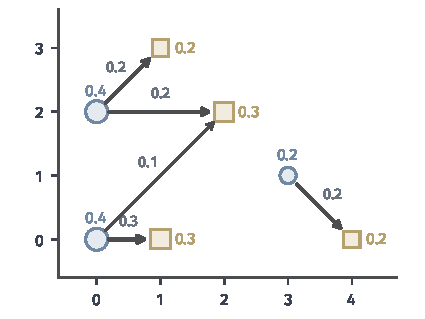
\includegraphics[width=72mm]{figures/07-probability/07-distribution-optimization/matplotlib/ot-lp-plane/figure.pdf}
 \caption{平面上的离散运输，平方欧氏成本。蓝圆是源点，黄方块是目标点，旁边的数是质量；箭头是最优方案的非零元，粗细与箭头旁的数表示搬运的质量。最优成本为$2.7$。}
 \label{fig:ot-lp-plane}
\end{BookInlineFigure}

\paragraph{结果的检验}
线性规划求解器输出的方案要逐项检验，不能只看目标值。检验三件事。第一，非负性：$\min_{i,j}\pi_{i,j}\geq0$。第二，边缘残差：行和与$\bm{a}$之差、列和与$\bm{b}$之差的$\ell_1$范数之和应为零，数值解应在容差以内；不满足边缘约束的方案，其成本不是最优值的上界。第三，原对偶差：再给出一对势$(\bm{f},\bm{g})$，检查对偶可行性$\max_{i,j}(f_i+g_j-c_{i,j})\leq0$，并计算$\langle\bm{C},\bm{\pi}\rangle-\langle\bm{a},\bm{f}\rangle-\langle\bm{b},\bm{g}\rangle$。由式~\eqref{eq:ot-gap}，前两项满足时这个差非负并且控制方案与最优值的距离。

对上面的例子，令$f_1=0$，在非零位置上解$f_i+g_j=c_{i,j}$，得$g_1=1$，$g_2=8$，$f_2=-4$，$g_4=6$；第三个源点只连$y_3$，自成一棵树，$f_3+g_3=2$还有一个自由度，取$f_3=-6$，$g_3=8$。于是
\[
 \bm{f}=(0,\ -4,\ -6),\qquad \bm{g}=(1,\ 8,\ 8,\ 6),
\]
松弛矩阵是
\[
 \bm{C}-\bigl(f_i+g_j\bigr)_{i,j}=\begin{bmatrix}0&0&8&4\\8&0&16&0\\10&0&0&8\end{bmatrix}\geq0 ,
\]
对偶值是
\[
 \langle\bm{a},\bm{f}\rangle+\langle\bm{b},\bm{g}\rangle=-2.8+5.5=2.7 ,
\]
原对偶差为零，$\bm{\pi}^{*}$最优。它也是唯一的最优方案：零松弛位置只有$(1,1),(1,2),(2,2),(2,4),(3,2),(3,3)$，第三列只有$(3,3)$一处零松弛，所以第三个源点的$0.2$必须全部给$y_3$，$(3,2)$只能为零；其余位置随之唯一确定。

\subsection{高斯分布的二次运输}
\label{sec:ot-gaussian}

在$\mathbb{R}^{d}$上取平方欧氏成本，$c(x,y)=\lVert x-y\rVert_2^{2}$。先把均值分离出去。设$X\sim\mu$，$Y\sim\nu$，均值分别是$\bm{m}_1,\bm{m}_2$，二阶矩有限，记$\tilde{X}=X-\bm{m}_1$，$\tilde{Y}=Y-\bm{m}_2$。对任意耦合，
\[
 \mathbb{E}\lVert X-Y\rVert_2^{2}=\lVert\bm{m}_1-\bm{m}_2\rVert_2^{2}+2\bigl\langle\bm{m}_1-\bm{m}_2,\ \mathbb{E}[\tilde{X}-\tilde{Y}]\bigr\rangle+\mathbb{E}\lVert\tilde{X}-\tilde{Y}\rVert_2^{2},
\]
中间项为零。所以平方运输成本等于均值之差的平方加上把两个中心化分布对齐的成本，两部分互不影响。中心化部分再展开，
\[
 \mathbb{E}\lVert\tilde{X}-\tilde{Y}\rVert_2^{2}=\operatorname{tr}\bm{\Sigma}_1+\operatorname{tr}\bm{\Sigma}_2-2\,\mathbb{E}\langle\tilde{X},\tilde{Y}\rangle ,
\]
其中$\bm{\Sigma}_1,\bm{\Sigma}_2$是协方差矩阵。前两项只依赖边缘，所以最小化成本就是最大化$\mathbb{E}\langle\tilde{X},\tilde{Y}\rangle$：让两个向量尽可能“同向”。

\begin{theorem}[高斯分布的平方运输]
\label{thm:ot-gaussian}
设$\mu=\mathcal{N}(\bm{m}_1,\bm{\Sigma}_1)$，$\nu=\mathcal{N}(\bm{m}_2,\bm{\Sigma}_2)$，两个协方差矩阵都正定。令
\begin{equation}
 \bm{A}=\bm{\Sigma}_1^{-1/2}\bigl(\bm{\Sigma}_1^{1/2}\bm{\Sigma}_2\bm{\Sigma}_1^{1/2}\bigr)^{1/2}\bm{\Sigma}_1^{-1/2},\qquad T(x)=\bm{m}_2+\bm{A}(x-\bm{m}_1).
 \label{eq:ot-gaussian-map}
\end{equation}
则$T$是从$\mu$到$\nu$的最优运输映射，并且
\begin{equation}
 W_2^{2}(\mu,\nu)=\lVert\bm{m}_1-\bm{m}_2\rVert_2^{2}+\operatorname{tr}\bm{\Sigma}_1+\operatorname{tr}\bm{\Sigma}_2-2\operatorname{tr}\bigl(\bm{\Sigma}_1^{1/2}\bm{\Sigma}_2\bm{\Sigma}_1^{1/2}\bigr)^{1/2}.
 \label{eq:ot-gaussian-w2}
\end{equation}
\end{theorem}

这里的平方根都是对称正定矩阵的唯一对称正定平方根。记$\bm{M}$为式~\eqref{eq:ot-gaussian-map}中括号的平方根，它对称正定；$\bm{A}$是对称正定矩阵与它的合同变换，仍对称正定。

\begin{proof}
\emph{映射可行。}$T$是仿射映射，$T(X)$是高斯向量，均值为$\bm{m}_2$，协方差为
\[
 \bm{A}\bm{\Sigma}_1\bm{A}=\bm{\Sigma}_1^{-1/2}\bm{M}\bm{\Sigma}_1^{-1/2}\bm{\Sigma}_1\bm{\Sigma}_1^{-1/2}\bm{M}\bm{\Sigma}_1^{-1/2}=\bm{\Sigma}_1^{-1/2}\bm{M}^{2}\bm{\Sigma}_1^{-1/2}=\bm{\Sigma}_2 .
\]
所以$T_\#\mu=\nu$。

\emph{映射最优。}由前面的分解，只需证明对中心化的任意耦合$(\tilde{X},\tilde{Y})$，内积的期望$\mathbb{E}\langle\tilde{X},\tilde{Y}\rangle$不超过$\tilde{Y}=\bm{A}\tilde{X}$时的值。对任意向量$x,y$，
\[
 \tfrac12\langle x,\bm{A}x\rangle+\tfrac12\langle y,\bm{A}^{-1}y\rangle-\langle x,y\rangle=\tfrac12\bigl\lVert\bm{A}^{1/2}x-\bm{A}^{-1/2}y\bigr\rVert_2^{2}\geq0 ,
\]
等号当且仅当$y=\bm{A}x$。代入$x=\tilde{X}$，$y=\tilde{Y}$并取期望，
\[
 \mathbb{E}\langle\tilde{X},\tilde{Y}\rangle\leq\tfrac12\operatorname{tr}(\bm{A}\bm{\Sigma}_1)+\tfrac12\operatorname{tr}(\bm{A}^{-1}\bm{\Sigma}_2).
\]
右边只依赖两个边缘，是一切耦合的公共上界；$\tilde{Y}=\bm{A}\tilde{X}$时取等，而这正是$T$给出的耦合。

\emph{成本。}在$T$给出的耦合下，$\mathbb{E}\langle\tilde{X},\bm{A}\tilde{X}\rangle$等于$\operatorname{tr}(\bm{A}\bm{\Sigma}_1)$，并且
\[
 \operatorname{tr}(\bm{A}\bm{\Sigma}_1)=\operatorname{tr}\bigl(\bm{\Sigma}_1^{-1/2}\bm{M}\bm{\Sigma}_1^{1/2}\bigr)=\operatorname{tr}\bm{M} .
\]
代入前面的分解即得式~\eqref{eq:ot-gaussian-w2}。
\end{proof}

证明中的二次型不等式是凸函数$\tfrac12\langle x,\bm{A}x\rangle$与它的凸共轭之间的Fenchel--Young不等式。一般地，平方成本下的最优映射是某个凸函数的梯度，这里的凸函数是二次函数，梯度就是对称正定的线性映射$\bm{A}$。对称性是关键：同样把$\mu$推成$\nu$的映射还有许多，但只有对称正定的那一个是最优的。

一维时式~\eqref{eq:ot-gaussian-w2}化为
\begin{equation}
 W_2^{2}\bigl(\mathcal{N}(m_1,\sigma_1^{2}),\mathcal{N}(m_2,\sigma_2^{2})\bigr)=(m_1-m_2)^{2}+(\sigma_1-\sigma_2)^{2},
 \label{eq:ot-gaussian-1d}
\end{equation}
最优映射是$T(x)=m_2+(\sigma_2/\sigma_1)(x-m_1)$，也就是第~\ref{sec:ot-one-dimensional}节的$G^{-1}\circ F$。

\paragraph{一个能手算的例子}
取$\mu=\mathcal{N}(\bm{0},\bm{I})$，$\nu=\mathcal{N}(\bm{m},\bm{\Sigma}_2)$，其中
\[
 \bm{m}=(3,\ 1),\qquad \bm{\Sigma}_2=\operatorname{diag}\bigl(4,\ \tfrac14\bigr).
\]
$\bm{\Sigma}_1=\bm{I}$，所以$\bm{A}=\bm{M}=\bm{\Sigma}_2^{1/2}$，即$\operatorname{diag}(2,\tfrac12)$，最优映射是
\[
 T(x)=(3,\ 1)+\bigl(2x_1,\ \tfrac12x_2\bigr).
\]
由式~\eqref{eq:ot-gaussian-w2}，
\[
 W_2^{2}=10+2+\tfrac{17}{4}-2\bigl(2+\tfrac12\bigr)=10+1.25=11.25 ,
\]
均值移动贡献$10$，形状改变贡献$(1-2)^{2}+(1-\tfrac12)^{2}=1.25$。

作为对照，先把$x$旋转$90^{\circ}$再拉伸：
\[
 T'(x)=\bm{m}+\operatorname{diag}\bigl(2,\tfrac12\bigr)\bm{R}x,\qquad \bm{R}=\begin{bmatrix}0&-1\\1&0\end{bmatrix}.
\]$\bm{R}\bm{R}^{\top}=\bm{I}$，所以$T'(X)$的协方差仍是$\bm{\Sigma}_2$，$T'$也是运输映射。它的成本是
\[
 10+\operatorname{tr}\bm{I}+\operatorname{tr}\bm{\Sigma}_2-2\operatorname{tr}\bigl(\operatorname{diag}(2,\tfrac12)\bm{R}\bigr)=10+2+4.25-0=16.25 .
\]
$\operatorname{diag}(2,\tfrac12)\bm{R}$不对称，对角线为零，它让$\tilde{X}$与$\tilde{Y}$完全不同向。图~\ref{fig:ot-gaussian-map}对比了两个映射：红点$(1,0)$在最优映射下送到$(5,1)$，在$T'$下送到$(3,\tfrac32)$。

\begin{BookInlineFigure}
 \centering
 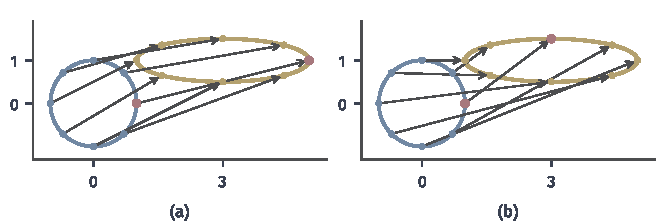
\includegraphics[width=112mm]{figures/07-probability/07-distribution-optimization/matplotlib/ot-gaussian-map/figure.pdf}
 \caption{$\mathcal{N}(\bm{0},\bm{I})$（蓝圈为单位标准差等高线）到$\mathcal{N}((3,1),\operatorname{diag}(4,\tfrac14))$（黄椭圆）。箭头是圆上八个点的像，红点是$(1,0)$及其像。(a)最优映射$T(x)=\bm{m}+\operatorname{diag}(2,\tfrac12)x$，成本$11.25$。(b)先旋转$90^{\circ}$再拉伸的映射，像分布相同，成本$16.25$。}
 \label{fig:ot-gaussian-map}
\end{BookInlineFigure}

\paragraph{奇异协方差}
定理要求$\bm{\Sigma}_1$可逆，因为$\bm{A}$的公式含$\bm{\Sigma}_1^{-1/2}$。源分布退化时，最优耦合与最优成本仍可研究，但必须按支撑子空间检查映射是否可行。取$d=2$，
\[
 \mu=\mathcal{N}\bigl(\bm{0},\operatorname{diag}(1,0)\bigr),\qquad \nu=\mathcal{N}(\bm{0},\bm{I}).
\]
$\mu$集中在横轴上，$X=(X_1,0)$。两者均值都是零，由前面的分解，最小化成本就是最大化$\mathbb{E}\langle X,Y\rangle$。对任意耦合，由Cauchy--Schwarz不等式，
\[
 \mathbb{E}\langle X,Y\rangle=\mathbb{E}[X_1Y_1]\leq\sqrt{\mathbb{E}X_1^{2}\,\mathbb{E}Y_1^{2}}=1 ,
\]
等号当且仅当$Y_1=X_1$。于是最优耦合必须让$Y_1=X_1$，而$Y_2$要服从$\mathcal{N}(0,1)$并且与$Y_1$独立（$\nu$的两个分量独立），所以最优耦合唯一：
\[
 Y=(X_1,\ Z),\qquad Z\sim\mathcal{N}(0,1)\ \text{与}\ X_1\ \text{独立},
\]
成本是$\mathbb{E}Z^{2}=1$。$Y_2$与$X$独立，不是$X$的函数，所以最优耦合不由映射产生，见图~\ref{fig:ot-gaussian-singular}。

反方向的问题落在定理~\ref{thm:ot-gaussian}之内。把两个分布对调，以$\nu$为源，它的协方差可逆，式~\eqref{eq:ot-gaussian-w2}给出
\[
 0+2+1-2\operatorname{tr}\operatorname{diag}(1,0)=1 ,
\]
与直接计算一致；对调方向的最优映射是投影$(y_1,y_2)\mapsto(y_1,0)$。协方差奇异时式~\eqref{eq:ot-gaussian-w2}本身仍然成立，可以用正定情形取极限得到，但不能把含$\bm{\Sigma}_1^{-1/2}$的映射公式直接套用。

\begin{BookInlineFigure}
 \centering
 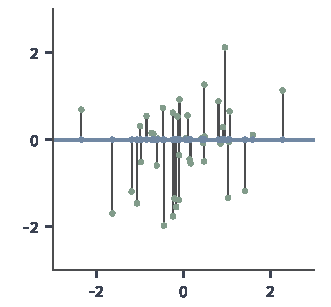
\includegraphics[width=56mm]{figures/07-probability/07-distribution-optimization/matplotlib/ot-gaussian-singular/figure.pdf}
 \caption{退化源分布$\mathcal{N}(\bm{0},\operatorname{diag}(1,0))$（蓝线为其支撑）到$\mathcal{N}(\bm{0},\bm{I})$的唯一最优耦合，$40$对模拟点，种子$729$。蓝点是源点，绿点是目标点，竖线是搬运路径：每份质量只沿竖直方向移动，目标高度与源点独立。}
 \label{fig:ot-gaussian-singular}
\end{BookInlineFigure}
